\documentclass[11pt,a4paper]{article}
\usepackage[T1]{fontenc}
\usepackage{graphicx}
\usepackage{mathtools}
\usepackage{amssymb}
\usepackage{geometry}
\usepackage{titlesec}
\usepackage{enumitem} % 添加enumitem宏包
\usepackage{amsfonts}
\usepackage{amssymb}
\usepackage{fancyhdr} % 添加fancyhdr宏包
\usepackage{lastpage} % 添加lastpage宏包
\usepackage{graphicx} % 导入graphicx包
\usepackage{gensymb} % 引入gensymb包
\usepackage[UTF8]{ctex}
% 应用fancyhdr宏包的页脚样式
\pagestyle{fancy}
\fancyhf{} % 清除当前的页眉页脚设置
\fancyfoot[L]{免费开源,请勿商用} % 页脚左下方显示文字
\fancyfoot[R]{作者:阿尧} % 页脚右下方显示文字
\renewcommand{\headrulewidth}{0pt} % 去掉页眉的横线
\renewcommand{\footrulewidth}{1pt} % 设置页脚的横线宽度
\usepackage{draftwatermark} %增加水印
\SetWatermarkText{本真题由b站up陈瀚尧探索世界免费开源}
\SetWatermarkScale{0.3} % 可以调整为合适的大小
\SetWatermarkColor{gray!50} % 灰色透明度为50%

% 设置更窄的页面边距
\geometry{left=3cm, right=3cm, top=1cm, bottom=2cm}

% 设置section标题格式
\titleformat{\title}{\bfseries}{\thetitle}{1em}{}

% 设置section之间的距离
\titlespacing*{\section}{0pt}{3.25ex plus 1ex minus .2ex}{1.5ex plus .2ex}

\begin{document}
    \title{中国科学院大学\\2015年招收攻读硕士学位研究生入学统一考试试题\\科目名称:光学}
    \author{制作者:b站up 陈瀚尧探索世界}
    \date{}
    \maketitle
    % 设置section标题不显示序号
    \titleformat{\section}[block]{\normalfont\Large\bfseries}{}{0pt}{}

    % 设置itemize环境的项目符号为空
    \setlist[itemize]{label=} 

    \section{考试须知:}
    \begin{itemize}[topsep=0pt,itemsep=0pt,partopsep=0pt]
        \item 1.本试卷满分为150分,全部考试时间总计180分钟。
        \vspace{-3mm}
        \item 2.所有答案必须写在答题纸上,写在试题纸上或草稿纸上一律无效。
        \vspace{-3mm}
        \item 3.可以使用无字典存储或编程功能的电子计算器。(此条对于25考研可能作废)
    \end{itemize}
    \vspace{-5mm}
    \noindent\rule{\textwidth}{0.5pt} % 添加一条线
    \vspace{-12mm}
    \section*{一、简答题(15分)}
    \begin{enumerate}
        \vspace{0mm}
        \item (1)解释光的直线传播定律、独立传播定律、反射定律和折射定律。
        \vspace{0mm}
        \item (2)解释焦点、焦平面、主点、主平面、节点。
        \vspace{0mm}
        \item (3)解释辐照度。
        \vspace{0mm}
        \item (4)解释孔径光阑、视场光阑、渐晕光阑、消杂光光阑。
        \vspace{0mm}
    \end{enumerate}
    \subsection*{2.如图,一薄透镜后 贴平面镜组成一个光学系统,物像同侧,u和v分别为物距和像距的绝对值,求a、b、c、d、e五种情况下该系统(包括薄透镜和平面镜)的组合焦距$f$,以及该薄透镜的焦距$f^{'}$,将结果填入下表:}
    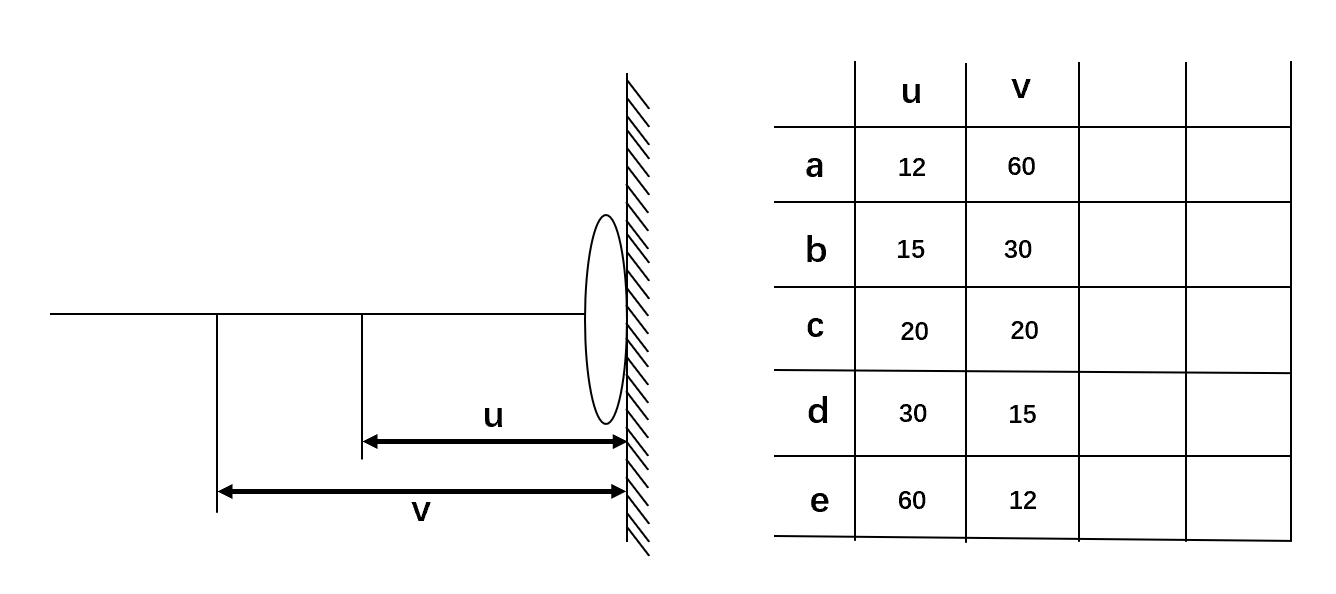
\includegraphics[scale=0.2]{1.png}% 插入图片,按50%的比例缩放
    \vspace{10mm}
    \subsection*{3.用口径为1m的光学望远镜的观察月球,能分辨月球表面上两点的最小距离是多少?(已知地月表面的距离是38万千米,假设光波长为$550nm$)}
    \vspace{10mm}
    \subsection*{4.显微镜目镜放大率为$15^{x}$,物镜放大率为$10^{x}$,求物镜、目镜焦距。光学筒长,组合焦距。}
    \vspace{10mm}
    \subsection*{5.今有光强为$I$的平行光束垂直入射二次等腰直角棱镜的斜面,被棱镜反射后,反向射出。若棱镜的折射率为1.52,不考虑棱镜的吸收,求棱镜的出射光强。}
    \vspace{10mm}
    \subsection*{6.一电矢量振动方向与入射面成$45\degree$的线偏振光以$60\degree$角入射到玻璃-空气界面上,玻璃和空气的折射率分别为1.5和1,试确定反射光的偏振状态。}
    \vspace{10mm}
    \subsection*{7.杨氏双缝干涉实验装置中,$S_1$,$S_2$间距为$d=0.45mm$,观察距离$r_0=45cm$,当如图以厚度$t=2.14*10^{-2}mm$折射率$n=1.56$的透明薄片贴住小孔$S_1$时,发现观察屏上的条纹产生移动,试确定条纹移动的方向和距离。}
    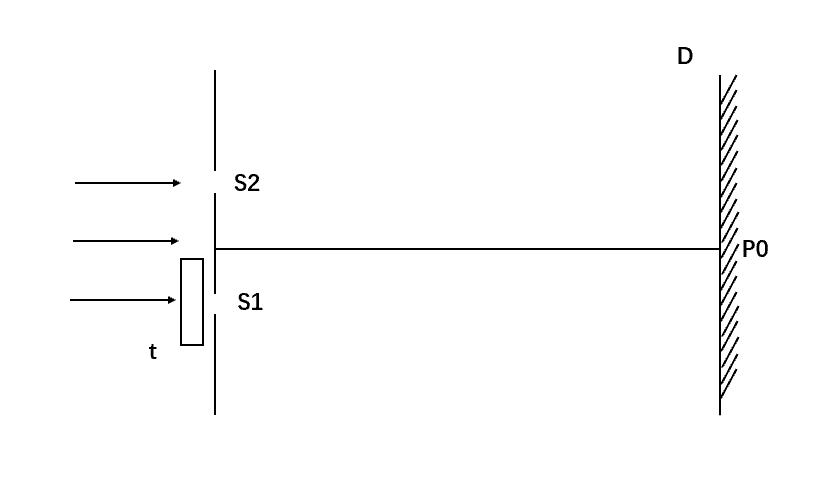
\includegraphics[scale=0.3]{2.png}% 插入图片,按50%的比例缩放
    \vspace{10mm}
    \subsection*{8.法布里-珀罗干涉仪的长度为5cm,腔镜的反射率为0.98。}
    \begin{itemize}
        \vspace{0mm}
        \item (1)用一波长为600nm的扩展光源照明该干涉仪,求其中心干涉条纹的级数和可分辨的最小波长间隔。
        \vspace{0mm}
        \item (2)若用一束波长范围为$380~780nm$,平行白光正入射该干涉仪,求输出纵膜的频率间隔和透射最强的谱线数目。
        \vspace{0mm}
    \end{itemize}
    \vspace{20mm}
    \subsection*{9.在正常条件下,人眼瞳孔直径约为2.5mm,人眼最灵敏波长为550nm。今有一台数值孔径约为0.9的显微镜:}
    \begin{itemize}
        \vspace{0mm}
        \item (1)试求它在$\lambda =550nm$可见光工作时的最小分辨距离。
        \vspace{0mm}
        \item (2)为充分利用显微镜这一分辨本领,显微镜放大率应设计成多大?
    \end{itemize}
    \vspace{20mm}
    \subsection*{10.一光栅宽10cm,每毫米内有500条刻线,试确定波长为$632.8nm$的平行光垂直入射时,第一级衍射光谱角半宽度和角色散。}
    \vspace{10mm}
    \subsection*{11.在两个偏振轴正交放置的偏振器之间平行放一块,慢轴方向折射率为0.0122的波片,偏振轴与波片快、慢轴夹角为$45\degree$,当入射光的波长$\lambda_1=0.583\mu m$时,视场全暗,进而逐渐改变光的波长;当$\lambda_2=0.554\mu m$时,视场又一次全暗,试求该波片的厚度。}
    \vspace{10mm}
    \subsection*{12.图中A为纵向运用的电光晶体KDP($n_o=1.512$,$r_63=10.6x10^{-10}\frac{cm}{v})$,B为厚度$d=15mm$的方解石晶体($n_o=1.5246$,$n_e=1.4792$),光轴方向与通光面法线方向成$45\degree$夹角。A、B晶体平行放置,试计算KDP晶体的半波电压$\frac{V}{2}$}
    \vspace{10mm}
    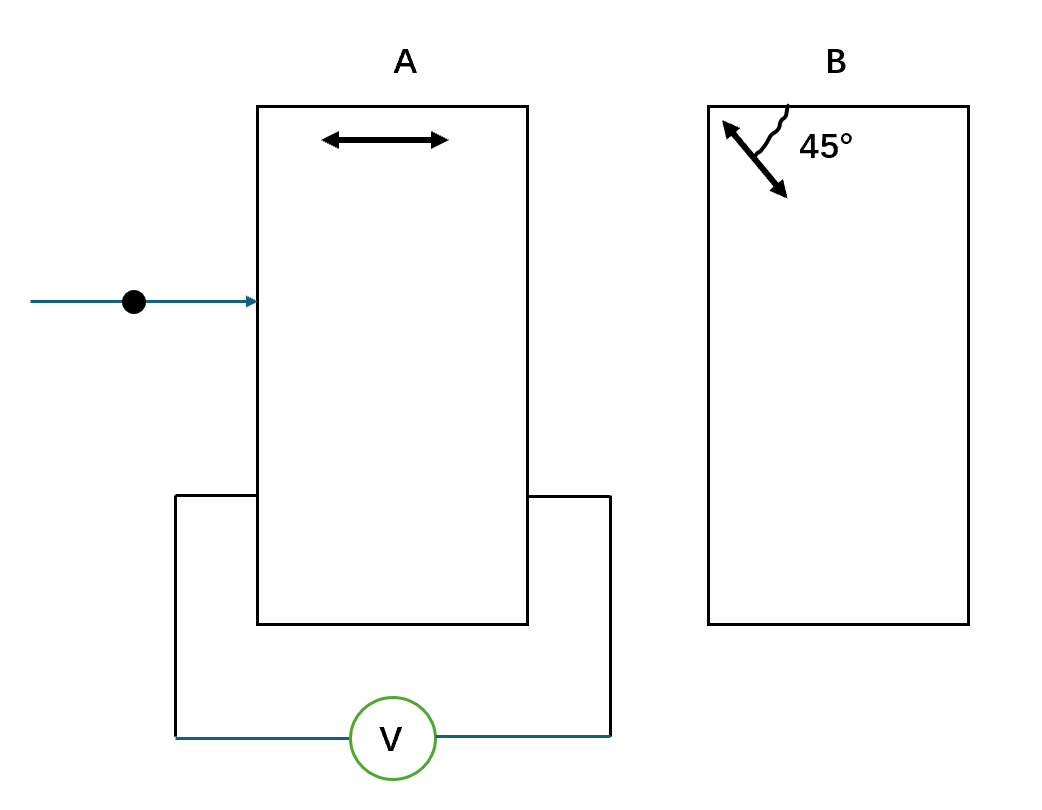
\includegraphics[scale=0.5]{3.jpg}% 插入图片,按50%的比例缩放
\end{document}